\documentclass[presentation]{beamer}
%\documentclass[presentation,aspectratio=169]{beamer}
%\documentclass[notes=only]{beamer}
%\documentclass[notes]{beamer}
\usetheme{default} %Pittsburgh %Rochester %Singapore
\usecolortheme{crane} %default 

%\DeclareUnicodeCharacter{0301}{*************************************}



% Graphics
\usepackage{caption}
\usepackage{subcaption}
\usepackage{graphicx}
\graphicspath{{figures/}}
\usepackage{float}

% Math
\usepackage{amssymb}
\usepackage{amsmath} % Required for some math elements 
\usepackage{numprint}

% Other
\usepackage{algorithmic}
\usepackage{array}
\usepackage{lipsum}
\usepackage{hyperref}

% code highlighting
\usepackage{listings}
\usepackage{color}

\definecolor{mygreen}{rgb}{0,0.6,0}
\definecolor{mygray}{rgb}{0.5,0.5,0.5}
\definecolor{mymauve}{rgb}{0.58,0,0.82}

\lstset{ %
  backgroundcolor=\color{white},   % choose the background color
  basicstyle=\footnotesize,        % size of fonts used for the code
  breaklines=true,                 % automatic line breaking only at whitespace
  captionpos=b,                    % sets the caption-position to bottom
  commentstyle=\color{mygreen},    % comment style
  escapeinside={\%*}{*)},          % if you want to add LaTeX within your code
  keywordstyle=\color{blue},       % keyword style
  stringstyle=\color{mymauve},     % string literal style
}
{}

% caption
%\usepackage{caption}
%\captionsetup[table]{font={small,stretch=0.5}, skip=5pt, position=above, labelfont=bf}
%\captionsetup[figure]{labelfont=bf}
\usepackage{booktabs}
\usepackage{siunitx}  
\sisetup{
    table-format = -1.3e-1,
    table-number-alignment = center,
    table-auto-round
  }

% reduce top margins of title
\addtobeamertemplate{frametitle}{}{\vspace{-1em}} % decrease

% adjust position of citation to bottom right and make them small
\newcommand{\mycite}{\hspace*{0.75\textwidth} \tiny \cite}
\newcommand{\secmycite}{\hspace*{0.5\textwidth} \tiny \cite}

% bibliography
\usepackage[style=authoryear,backend=bibtex]{biblatex}
\renewcommand*{\bibfont}{\small}
%\bibliography{bibliography/sources}
\addbibresource{bibliography/sources.bib}
\usepackage[absolute,overlay]{textpos}
\usepackage{calc}


% reduce control elements (compared to default)
\setbeamertemplate{navigation symbols}{\insertslidenavigationsymbol}

%Information to be included in the title page:
\title{SAveRUNNER: COVID-19}
%\subtitle{Digital Epidemiology and Precision Medicine}
\author{ \fontsize{18}{50}\selectfont Sean Klein}
\institute{\fontsize{10}{50}\selectfont Digital Epidemiology and Precision Medicine}
\date{\fontsize{10}{50}\selectfont Winter Semester 2021/22}



\begin{document}

\frame{\titlepage}

\begin{frame}
\frametitle{Setup}

\begin{itemize}
    \item SAveRUNNER 
    \begin{itemize}
        \item p-value threshold of $0.05$
        \item Network: COVID-19 \& SARS
        \item Subnetwork: COVID-19
    \end{itemize}
    \item TTD associations
    \item Cytoscape: Network of common drugs (SARS \& COVID-19)
\end{itemize}

\end{frame}

% ---------------------------------
\setbeamertemplate{footline}[text line]{%
\parbox{\linewidth}{\vspace*{-8pt}\insertsection\hfill\insertpagenumber}} %\insertshortauthor\hfill

\section{SAveRUNNER Output}
\begin{frame}{Disease-Disease heatmap}
    \begin{figure}
         \centering
         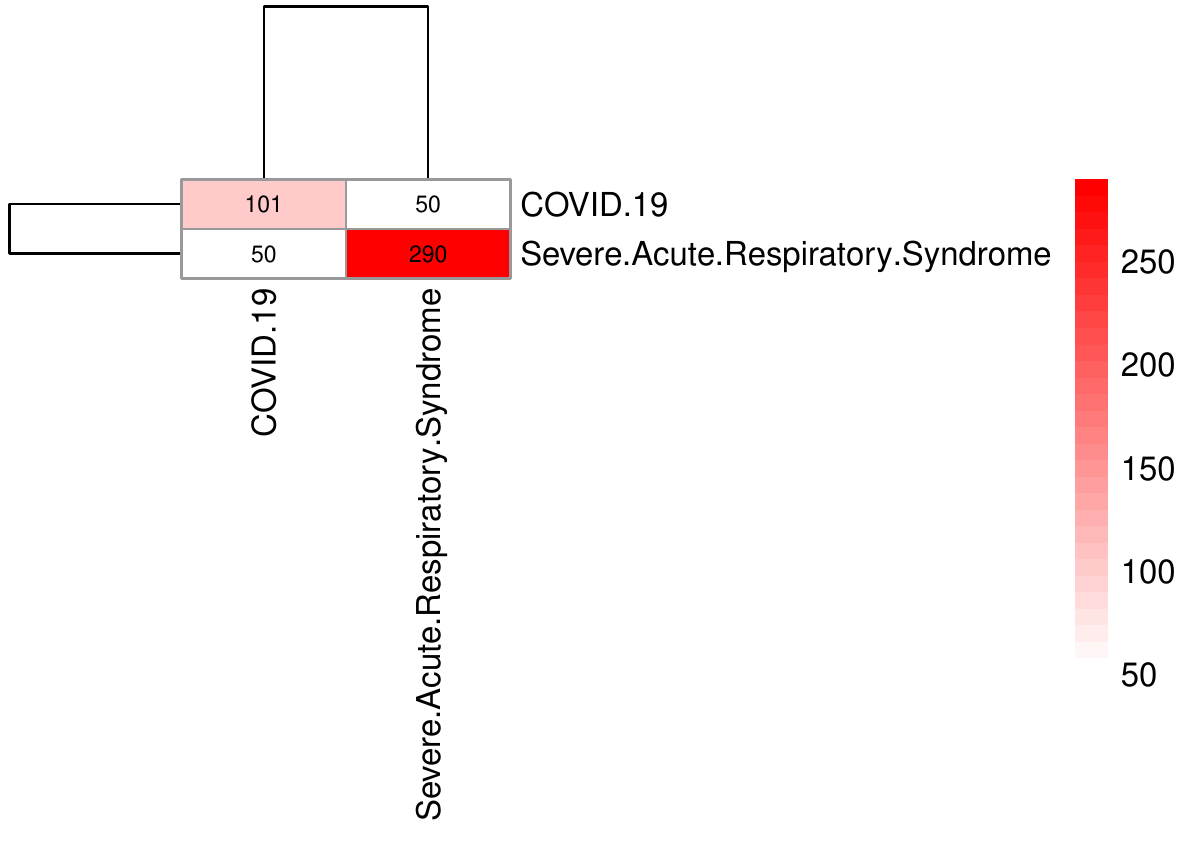
\includegraphics[scale=0.33]{figures/Disease_Disease_Heatmap.png}
         %\caption{clustered heatmap visualizing amount of shared  drugs between diseases.}
         \label{fig:DieseaseDiesease}
     \end{figure}
\end{frame}

\begin{frame}{Repurposable drugs}
    \begin{table}%[H]
        \begin{center}
    
        %\captionsetup{width=10.5cm}
        %\caption{Predicted repurposable drugs for COVID-19. Values are sorted by p-values and are also rounded to three decimals. Only the drugs with 20 lowest p values are shown.}
        %\label{tab:predDrugsCovid}
        \npdecimalsign{.}
        \begin{tabular}{ l S S }
        \toprule
        \text{Drug} & \text{p-Value} & \text{Adjusted Similarity} \\
        \midrule
        azacitidine     & 1.698e-07 & 1.000e+00             \\
        riboflavin      & 1.910e-06 & 9.932e-01             \\
        noscapine       & 9.400e-06 & 1.000e+00             \\
        phylloquinone   & 1.288e-05 & 9.994e-01             \\
        \bottomrule
        \end{tabular}
        \npnoround
        
        \end{center}
    \end{table}
    
    \begin{itemize}
        %\item Sorted by p-value: only 4 lowest out of 50
        \item Azacitidine - concurrent acute myeloid leukemia 
        \item Riboflavin + UV - lowers c(SARS-CoV-2) 
        \item Noscapine - symptomatic treatment 
        \item Phylloquinone - Vitamin K1; impacts cytokine storm 
        
    \end{itemize}
    
    \vfill
    \tiny  {\parencite{Taurino_2021, Ragan_2020, Yonemura_2021, Wishart2017, Popa_2021, Dofferhoff_2020}} %\cite{Taurino_2021, Ragan_2020, Yonemura_2021, Wishart2017, Popa_2021, Dofferhoff_2020}
    \vspace*{0.1cm}

\end{frame}

\section{TTD associations}
\begin{frame}{Most common on-label targets}

    \begin{figure}
        \centering
        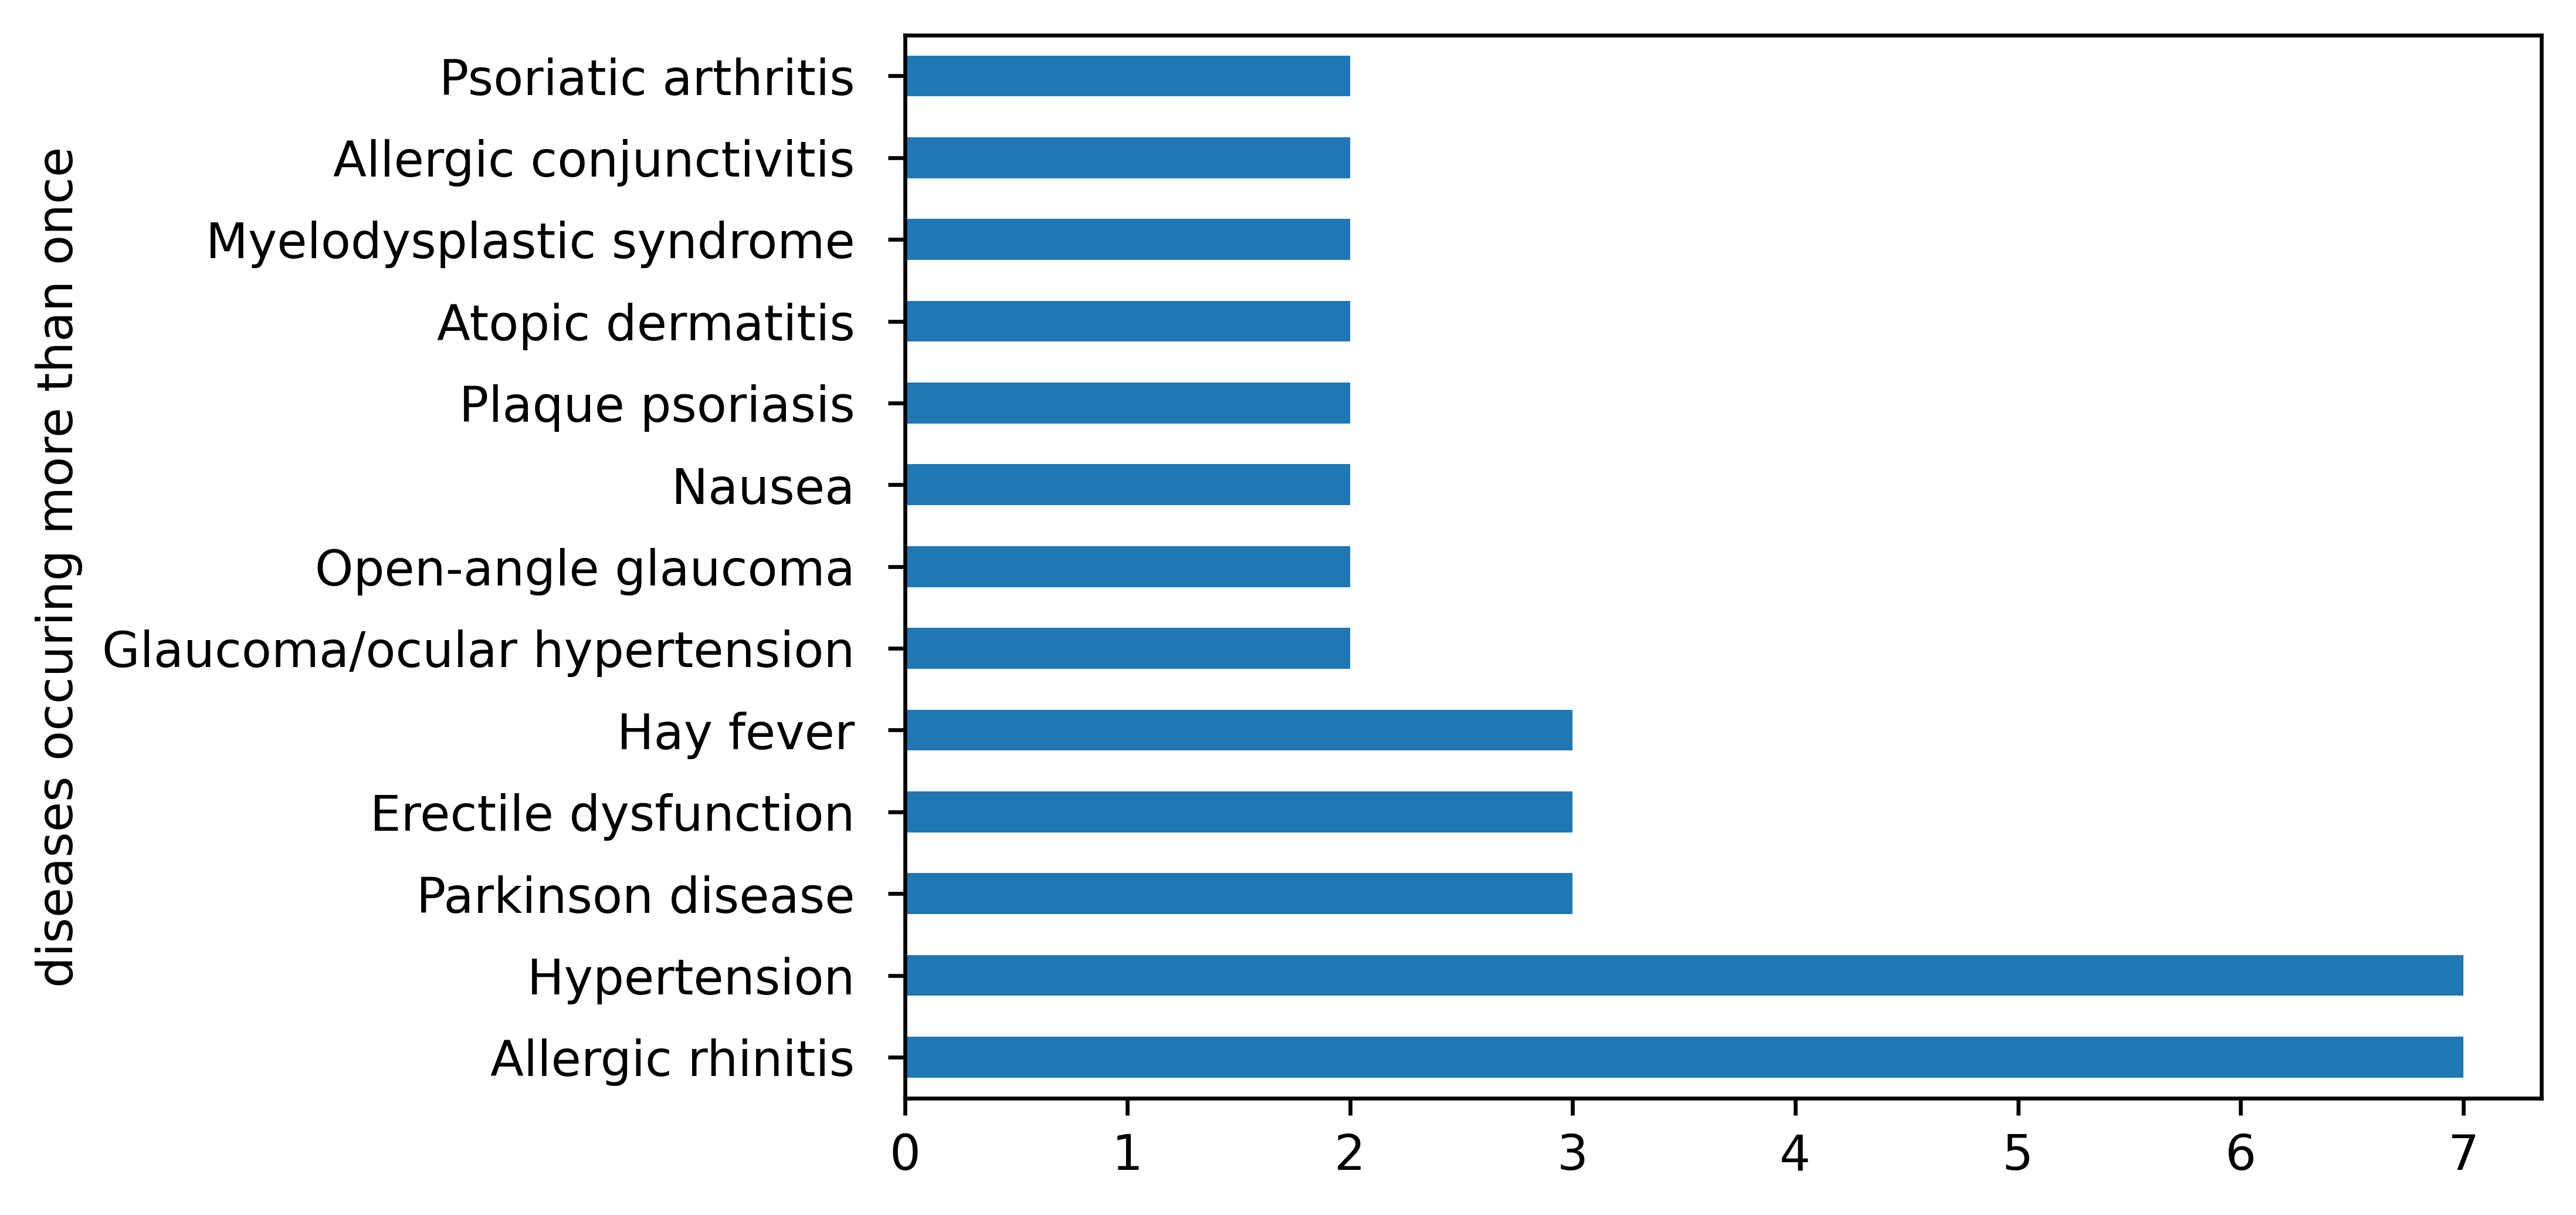
\includegraphics[width=0.8\textwidth]{figures/onLabel_diseases_saverunner_covid.png}
    \end{figure}

    \begin{itemize}
        \item Hypertension - ACE inhibiting drugs
        \item Allergic rhinitis - Histamine receptor H1/ immune system
    \end{itemize}
    
    \vfill
    %\vspace*{0.5cm}
    \tiny {\parencite{Wishart2017, Kim_2021, Chiu_2021}} %\cite{Wishart2017, Kim_2021, Chiu_2021}
    \vspace*{0.1cm}
    
\end{frame}


\section{SARS Overlap}
\begin{frame}{Network - Spring embedded layout}
    \begin{figure}
        \centering
        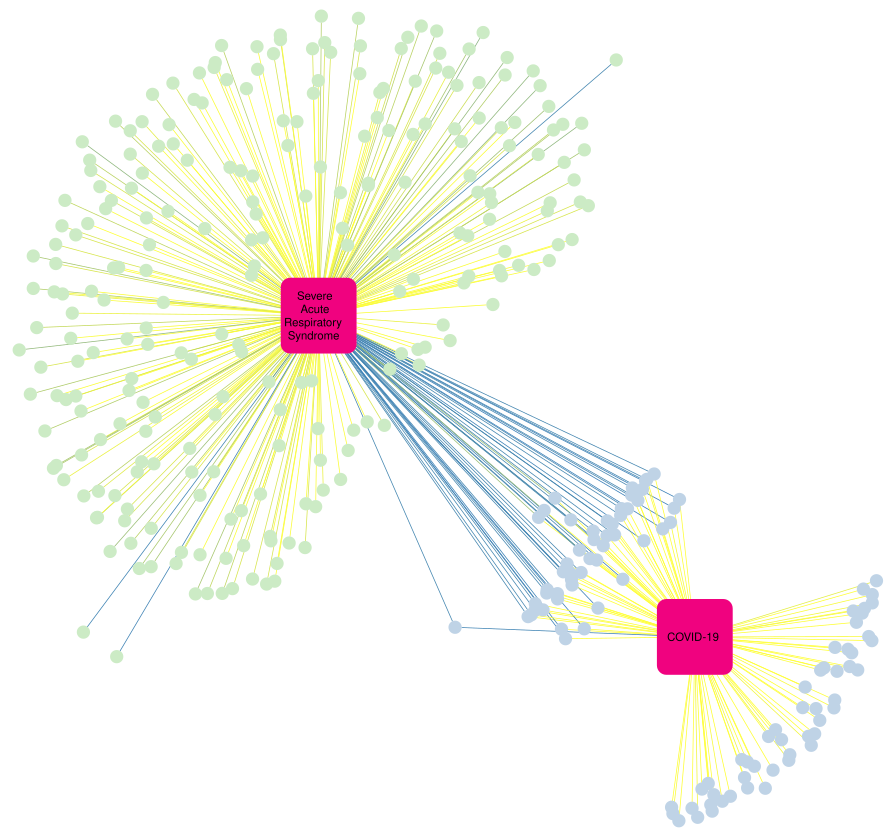
\includegraphics[scale=0.33]{figures/COVID19xSARS_network.png}
    \end{figure}
\end{frame}

\begin{frame}{High adjusted similarity shared}
    \begin{table}[H]
    \begin{center}
    
    \npdecimalsign{.}
    \nprounddigits{3}
    \begin{tabular}{ l n{2}{5} n{2}{5} n{2}{5}}
    \toprule
    \text{Drug} & \text{COVID-19} & \text{SARS} & \text{Sum} \\
    \midrule
    \text{benazepril}  & 0.9932432669830258 & 0.504781792120694 & 1.4980250591037199  \\
    \text{cilazapril} & 0.9932432669830258 & 0.504781792120694 & 1.4980250591037199  \\
    \text{quinapril} & 0.9932432669830258 & 0.504781792120694 & 1.4980250591037199  \\
    \text{turoctocog alfa pegol} & 0.9932432669830258 & 0.161441849724981   & 1.1546851167080068 \\
    \bottomrule
    \end{tabular}
    \npnoround
    
    \end{center}
    \end{table}
    
    \begin{itemize}
        \item Benazepril, Cilazapril \& Quinapril - ACE inhibitors
        \item Turoctocog alfa pegol - Haemophilia
    \end{itemize}
    
    \vfill \tiny  {\parencite{Wishart2017}} %\cite{Wishart2017}
    %\vspace*{0.1cm}
    
\end{frame}

\section{}
\begin{frame}[allowframebreaks, noframenumbering, c, plain]%{Thank you for your attention!}

%\bibliography{bibliography/sources.bib}
\printbibliography
%\vspace{0.5cm}
\end{frame}

\end{document}